\documentclass[tikz, border=5pt]{standalone}

\begin{document}

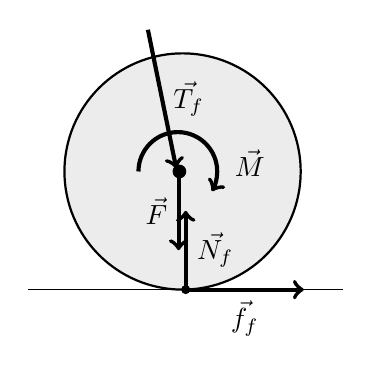
\begin{tikzpicture}

    %% FBD of Front wheel
    % Front wheel
    \draw[thick, fill=gray!15] (-0.04,0) circle(1.5);
    \draw[fill] (-0.08,0) circle(0.08);

    % Normal force
    \draw[->, line width=1.5pt] (0,-1.5) -- (0,-0.5) node[midway,right] {$\vec{N_f}$};
    \draw[fill] (0,-1.5) circle(0.05);

    % Applied force on the pedal
    \draw[->, line width=1.5pt] (-0.09,0) -- (-0.09,-1) node[midway,left] {$\vec{F}$};

    % Frictional force
    \draw[->, line width=1.5pt] (0,-1.5) -- (1.5,-1.5) node[midway,below] {$\vec{f_f}$};

    % Chassis force
    \draw[->, line width=1.5pt] (-0.48,1.8) -- (-0.08-0.04,0+0.04) node[midway, right] {$\vec{T_f}$};

    % Moment due to the applied force
    \draw[->, line width=1.5pt] (-0.6,0) arc[start angle=180, end angle=-30, radius=0.5];
    \node [right] at (0.5,0.1) {$\vec{M}$};

    % Ground
    \draw (-2,-1.5) -- (2,-1.5);

\end{tikzpicture}

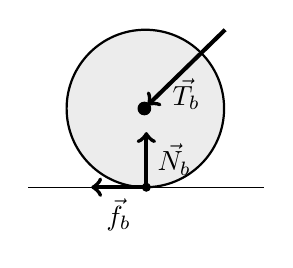
\begin{tikzpicture}

    %% FBD of Back wheel
    % Back wheel
    \draw[thick, fill=gray!15] (-0.0125,0) circle(1);
    \draw[fill] (-0.025,0) circle(0.08);

    % Normal force
    \draw[->, line width=1.5pt] (0,-1) -- (0,-0.3) node[midway,right] {$\vec{N_b}$};
    \draw[fill] (0,-1) circle(0.05);

    % Frictional force
    \draw[->, line width=1.5pt] (0,-1) -- (-0.7,-1) node[midway,below] {$\vec{f_b}$};

    % Chassis force
    \draw[->, line width=1.5pt] (1,1) -- (-0.025+0.04,0+0.04) node[midway, below] {$\vec{T_b}$};

    % Ground
    \draw (-1.5,-1) -- (1.5,-1);

\end{tikzpicture}

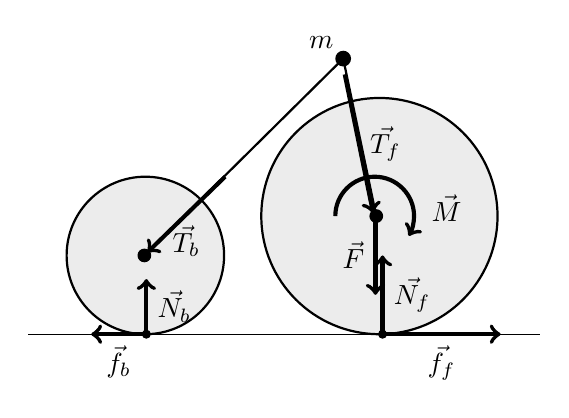
\begin{tikzpicture}

    %% FBD of Entire Bicycle
    \begin{scope}
        % Front wheel
        \draw[thick, fill=gray!15] (-0.04,0) circle(1.5);
        \draw[fill] (-0.08,0) circle(0.08);

        % Normal force
        \draw[->, line width=1.5pt] (0,-1.5) -- (0,-0.5) node[midway,right] {$\vec{N_f}$};
        \draw[fill] (0,-1.5) circle(0.05);

        % Applied force on the pedal
        \draw[->, line width=1.5pt] (-0.09,0) -- (-0.09,-1) node[midway,left] {$\vec{F}$};

        % Frictional force
        \draw[->, line width=1.5pt] (0,-1.5) -- (1.5,-1.5) node[midway,below] {$\vec{f_f}$};

        % Chassis force
        \draw[->, line width=1.5pt] (-0.48,1.8) -- (-0.08-0.04,0+0.04) node[midway, right] {$\vec{T_f}$};

        % Moment due to the applied force
        \draw[->, line width=1.5pt] (-0.6,0) arc[start angle=180, end angle=-30, radius=0.5];
        \node [right] at (0.5,0.1) {$\vec{M}$};
    \end{scope}
    \begin{scope}[xshift=-3cm, yshift=-0.5cm]
        % Back wheel
        \draw[thick, fill=gray!15] (-0.0125,0) circle(1);
        \draw[fill] (-0.025,0) circle(0.08);

        % Normal force
        \draw[->, line width=1.5pt] (0,-1) -- (0,-0.3) node[midway,right] {$\vec{N_b}$};
        \draw[fill] (0,-1) circle(0.05);

        % Frictional force
        \draw[->, line width=1.5pt] (0,-1) -- (-0.7,-1) node[midway,below] {$\vec{f_b}$};

        % Chassis force
        \draw[->, line width=1.5pt] (1,1) -- (-0.025+0.04,0+0.04) node[midway, below] {$\vec{T_b}$};
    \end{scope}

    % Ground
    \draw (-4.5,-1.5) -- (2,-1.5);

    % Chassis
    \draw[thick] (-0.08,0) -- (-0.5,2);
    \draw[thick] (-0.5,2) -- (-3.025,-0.5);

    % Rider
    \fill (-0.5,2) circle(0.1);
    \node [left] at (-0.5,2.2) {\(m\)};

\end{tikzpicture}

\end{document}
